\documentclass[9pt]{article}
\usepackage{graphicx} % Required for inserting images
\usepackage{tabularx}
\usepackage{hyperref}
\usepackage{makecell}
\usepackage{makeidx}
\usepackage{eurosym}
\usepackage{fancyhdr}
\usepackage{titlesec}
\usepackage[export]{adjustbox}
\usepackage{float}
\newcommand{\firstPage}{
    \thispagestyle{empty}
    \begin{figure}
    \centering
    
\includegraphics[scale=0.7]{Swellfish_logo.png}
    \end{figure}
    \author{
        \date{}
        \href{mailto://swellfish14@gmail.com}{swellfish14@gmail.com} \\
    } 
} 
\usepackage{hyperref}
\usepackage{array}
\usepackage{tabularx}
\usepackage{adjustbox}

\newcounter{verscount}
\setcounter{verscount}{0}
\newcommand{\addversione}[5]{
	\ifdefined\setversione
		\setversione{#1}
	\else\fi
	\stepcounter{verscount}
	\expandafter\newcommand%
		\csname ver\theverscount \endcsname{#1&#2&#3&#4&#5}
}

\newcommand{\listversioni}{
	\ifnum\value{verscount}>1
		\csname ver\theverscount \endcsname
		\addtocounter{verscount}{-1}
		\\\hline
		\listversioni
	\else
		\csname ver\theverscount \endcsname\\\hline
	\fi
}

\newcommand{\makeversioni}{
	\begin{center}
		\begin{tabularx}{\textwidth}{|c|c|X|X|X|}
		\hline
		\textbf{Versione} & \textbf{Data} & \textbf{Redattore} & \textbf{Verificatore} & \textbf{Descrizione} \\
		\hline
		\listversioni
		\end{tabularx}
	\end{center}
	\clearpage
}

\fancypagestyle{genericDocstyle}{
	\pagestyle{fancy}
	\lhead{
\includegraphics[width=1cm]{Swellfish_logo.png}}
	\rhead{Norme di progetto}
}

%\hypersetup{colorlinks=true,urlcolor=blue}

%\newcommand{\tableContent}{

	%{
		%\hypersetup{linkcolor=black}
		%\tableofcontents
	%}
%}

\begin{document}
\graphicspath{ {../templates/img/} {./img}}
\setcounter{tocdepth}{4}
\setcounter{secnumdepth}{4}
\title{Manuale Utente}

\firstPage
\maketitle

\begin{center}
	\begin{tabular}{r | l}
		\multicolumn{2}{c}{\textit{Informazioni}}        \\
		\hline

		\textit{Redattori}    &
		[Claudio Giaretta, Francesco Naletto]\makecell{} \\

		\textit{Revisori}     &
		[Jude Vensil Barceros]\makecell{}                \\
		\textit{Responsabili} &
		[Andrea Veronese]\makecell{}                     \\
		\textit{Uso}          &
		[Esterno]\makecell{}                             \\
	\end{tabular}
\end{center}

\begin{center}
	\textbf{Descrizione}\\
	File contenente Questo documento racchiude le istruzioni per l’utilizzo corretto di LumosMinima
\end{center}

\pagebreak

\printindex
\pagebreak

\tableofcontents
\pagebreak

\addversione{0.0.0}{23/08/2023}{Davide Porporati}{Claudio Giaretta}{Impostata struttura documento}
\addversione{0.0.1}{04/09/2023}{Francesco Naletto}{Claudio Giaretta}{Redatta prima versione documento}
\addversione{0.0.2}{09/09/2023}{Davide Porporati}{Elena Marchioro}{Completato documento}
\addversione{1.0.0}{09/09/2023}{Davide Porporati}{Elena Marchioro}{Aggiornato le immagini in base al CSS e revisionato}
\addversione{1.0.1}{20/09/2023}{Davide Porporati}{Elena Marchioro}{Aggiunte sezioni simulatori}

\makeversioni

\section{Introduzione}
\subsection{Scopo del documento}
Il presente documento ha lo scopo di delineare le funzioni offerte dall'applicazione e di fornire istruzioni dettagliate per l'utente sull'uso di quest'ultima.
In tal modo, l'utente verrà informato sui requisiti minimi indispensabili per assicurare il corretto funzionamento di LumosMinima.
\subsection{Cos'è LumosMinima}
LumosMinima è un progetto che mira a ottimizzare l'illuminazione pubblica. L'obiettivo è regolare l'intensità luminosa degli impianti pubblici al fine di garantire sicurezza e risparmio energetico. Il sistema agisce automaticamente sui dispositivi di illuminazione, rileva la presenza umana, segnala guasti e offre un controllo globale dell'intensità luminosa. LumosMinima rappresenta una soluzione innovativa per affrontare le sfide energetiche e ambientali del futuro.

\section{Strumenti necessari}
Per garantire il corretto funzionamento dell'applicazione, è indispensabile avere una connessione internet attiva. L'applicazione è stata verificata e supporta i seguenti browser:

\begin{itemize}
	\item Chrome, versione 116.
	\item Safari, versione 16.5.
	\item Edge, versione 116.
	\item Firefox, versione 117.
	\item Opera, versione 102.
\end{itemize}
\clearpage
\section{Installazione}
Per poter utilizzare il software LumosMinima, è necessario scaricare i file sorgene dalla repository del gruppo.

Una volta scaricata la cartella è necessario effettuare la build del frontend e del backend e importare infine il database in formato SQL.

\subsection{Build e avvio del frontend}
Per avviare il frontend, i seguenti passi sono necessari:
\begin{itemize}
	\item spostarsi sulla cartella "Lumosminima", utilizzando il comando "cd Lumosminima"
	\item spostarsi nel frontend, utilizzando il comando "cd client"
	\item eseguire la build, utilizzando il comando "npm build". Questo comando installerà in automatico tutte le dipendenze necessarie all'applicazione.
	\item avviare il client, digitando "npm start". Questo comando avvierà la Gui, e avvierà automaticamente il browser alla pagina "localhost:3000".
\end{itemize}
\subsection{Importazione del Database}
L'avvio del server contenente il database è un prerequisito fondamentale per il corretto funzionamento del backend dell'applicazione, pertanto va effettuato prima di avviare la componente server del sistema.
Per importare il database i seguenti passi sono necessari:
\begin{itemize}
	\item spostarsi sulla cartella "DB", utilizzando il comando "cd Db"
	\item importare il file "lumos-minima-pb.sql"nell'applicativo per la gestione e l'avvio dei database. Importando questo file viene creato un server al cui interno vengono importate le tabelle e i dati necessarie al funzionamento dell'applicazione.
\end{itemize}
\subsection{Build e avvio del backend}
Per avviare il backend, i seguenti passi sono necessari:
\begin{itemize}
	\item spostarsi sulla cartella "Lumosminima", utilizzando il comando "cd Lumosminima"
	\item spostarsi nel backend, utilizzando il comando "cd server"
	\item eseguire la build, utilizzando il comando "npm build". Questo comando installerà in automatico tutte le dipendenze necessarie all'applicazione.
	\item avviare il server, digitando "node indexPb.js". Questo comando avvia il server.
\end{itemize}

\subsection{Simulazione lampioni}
Per simulare i lampioni a sistema è necessario utilizzare il file "lamp-simulator-multiprocessing.py" presente nella cartella "simulatori".
Questo script Python si appoggia ad un file in formato JSON che contiene tutti i lampioni presi direttamente dal Database.

Per avviare il simulatore occorre eseguire i seguenti passi:
\begin{itemize}
	\item caricare i lampioni in formato JSON nel file "lamps.json"
	\item aprire un terminale ed esegure il comando "cd Simulatori"
	\item eseguire lo script python con il seguente comando "python ./lamp-simulator-multiprocessing.py". Questo comando istanzia i simulatori dei lampioni a sistema.
\end{itemize}

\subsection{Simulazione sensore}
Per simulare un sensore il procedimento è il seguente:
\begin{itemize}
	\item aprire un terminale ed esegure il comando "cd Simulatori"
	\item eseguire lo script python con il seguente comando "python ./sensor-simulator.py". 
	\item Aggiungere i parametri desiderati per l'istanziazione di un sensore: "-i" e seguito dall'id del sensore, "-s " seguito da 0 o 1 per indicare l'assenza o la presenza di un rilevamento, "-r" seguito dal range in metri di rilevamento, "-p" indica la porta in cui il sensore è in ascolto. Infine inserire "-a" e l'id dell'area illuminata di afferenza.
\end{itemize}
Al termine della procedura il sensore è operativo.
\section{LumosMinima}
\subsection{Home}
Il sito LumosMinima si presenta con una dashboard composta di 4 pannelli che danno informazioni generali
sul sistema

\begin{center}
	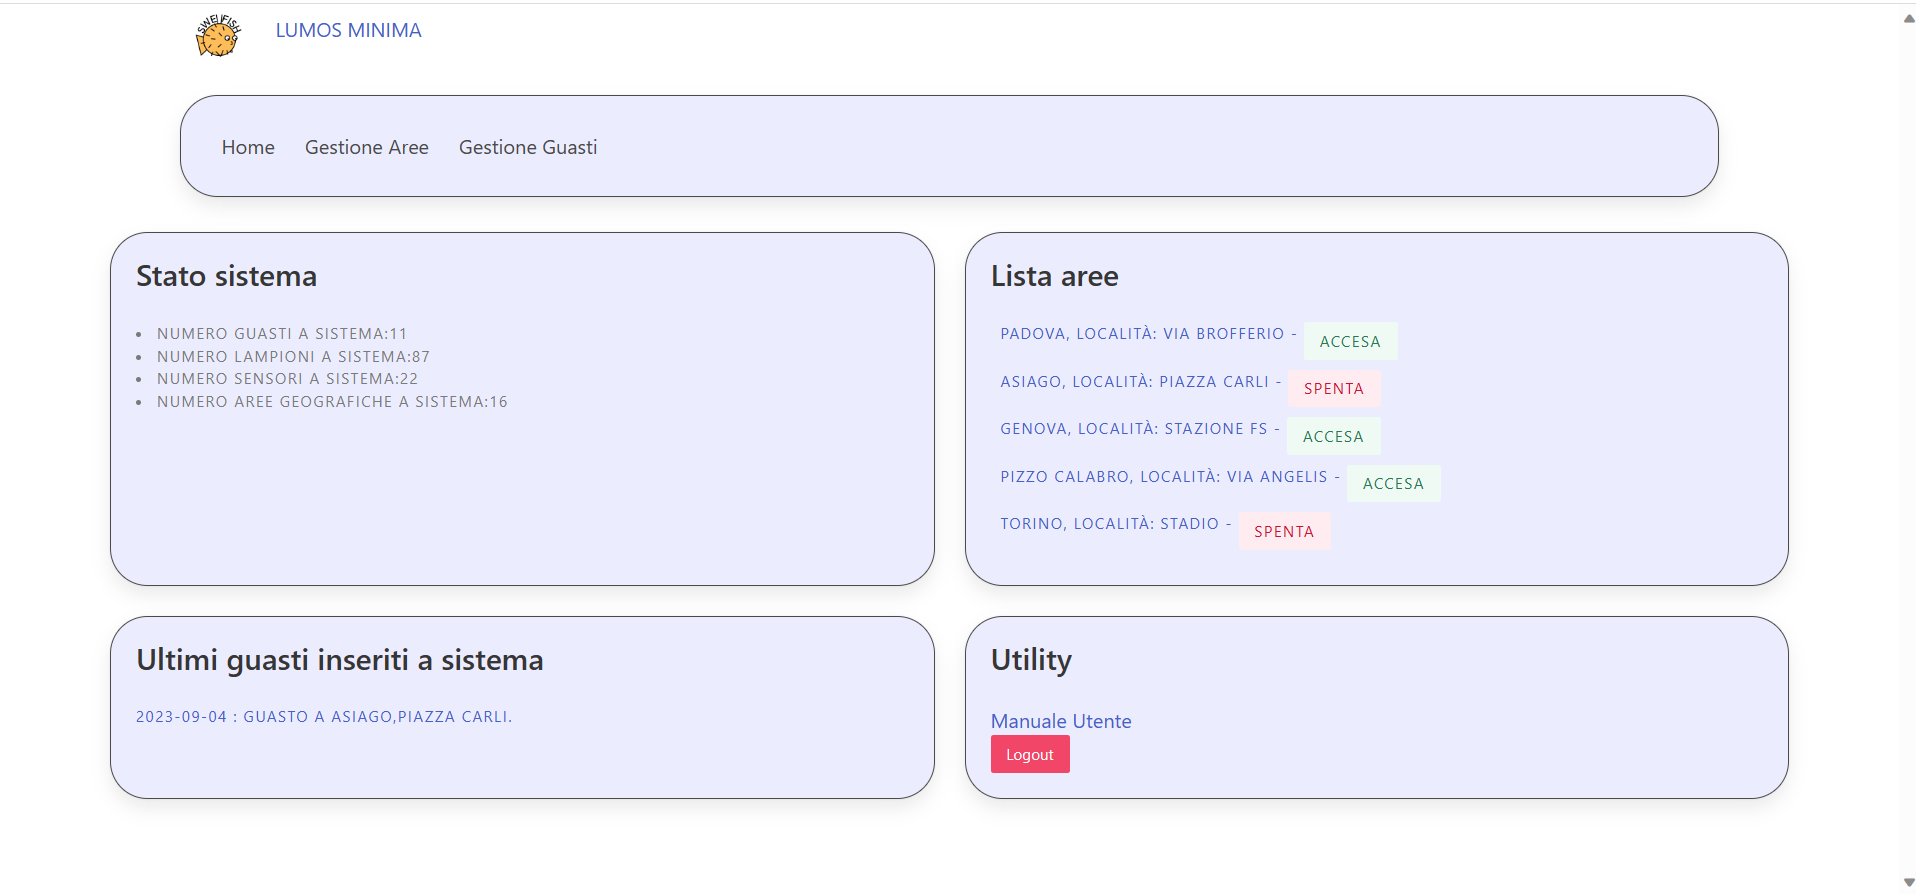
\includegraphics[scale=0.3]{LumosMinimaHome.png}
\end{center}

In particolare:
\begin{itemize}
	\item \textbf{Riquadro in alto a sinistra}: indica informazioni riguardanti lo stato del sistema
	\item \textbf{Riquadro in alto a destra}: riporta una lista limitata delle aree illuminate inserite a sistema
	\item \textbf{Riquadro in basso a sinistra}: riporta una lista delle ultime segnalazioni di guasti inseriti a sistema dall'utente
	\item \textbf{Riquadro in basso a destra}: riporta un link in cui è possibile scaricare il manuale utente e un pulsante per effettuare il logout dal sistema\\
\end{itemize}

La navbar presente in alto è composta da 3 link:

\begin{itemize}
	\item \textbf{Home}: Porta alla pagina corrente ovvero la Home
	\item \textbf{Gestione aree}: porta alla pagina "Gestione Aree" in cui è possibile gestire le varie aree inserite a sistema
	\item \textbf{Gestione guasti}: porta alla pagina in cui vengono visualizzati tutti i guasti segnalati a sistema
\end{itemize}

\subsection{Gestione aree}
In questa pagina è presente la lista di tutte le aree inserite a sistema.
Ogni area ha un tasto associato che porta alla pagina di dettaglio corrispondente all'area cliccata.

\begin{center}
	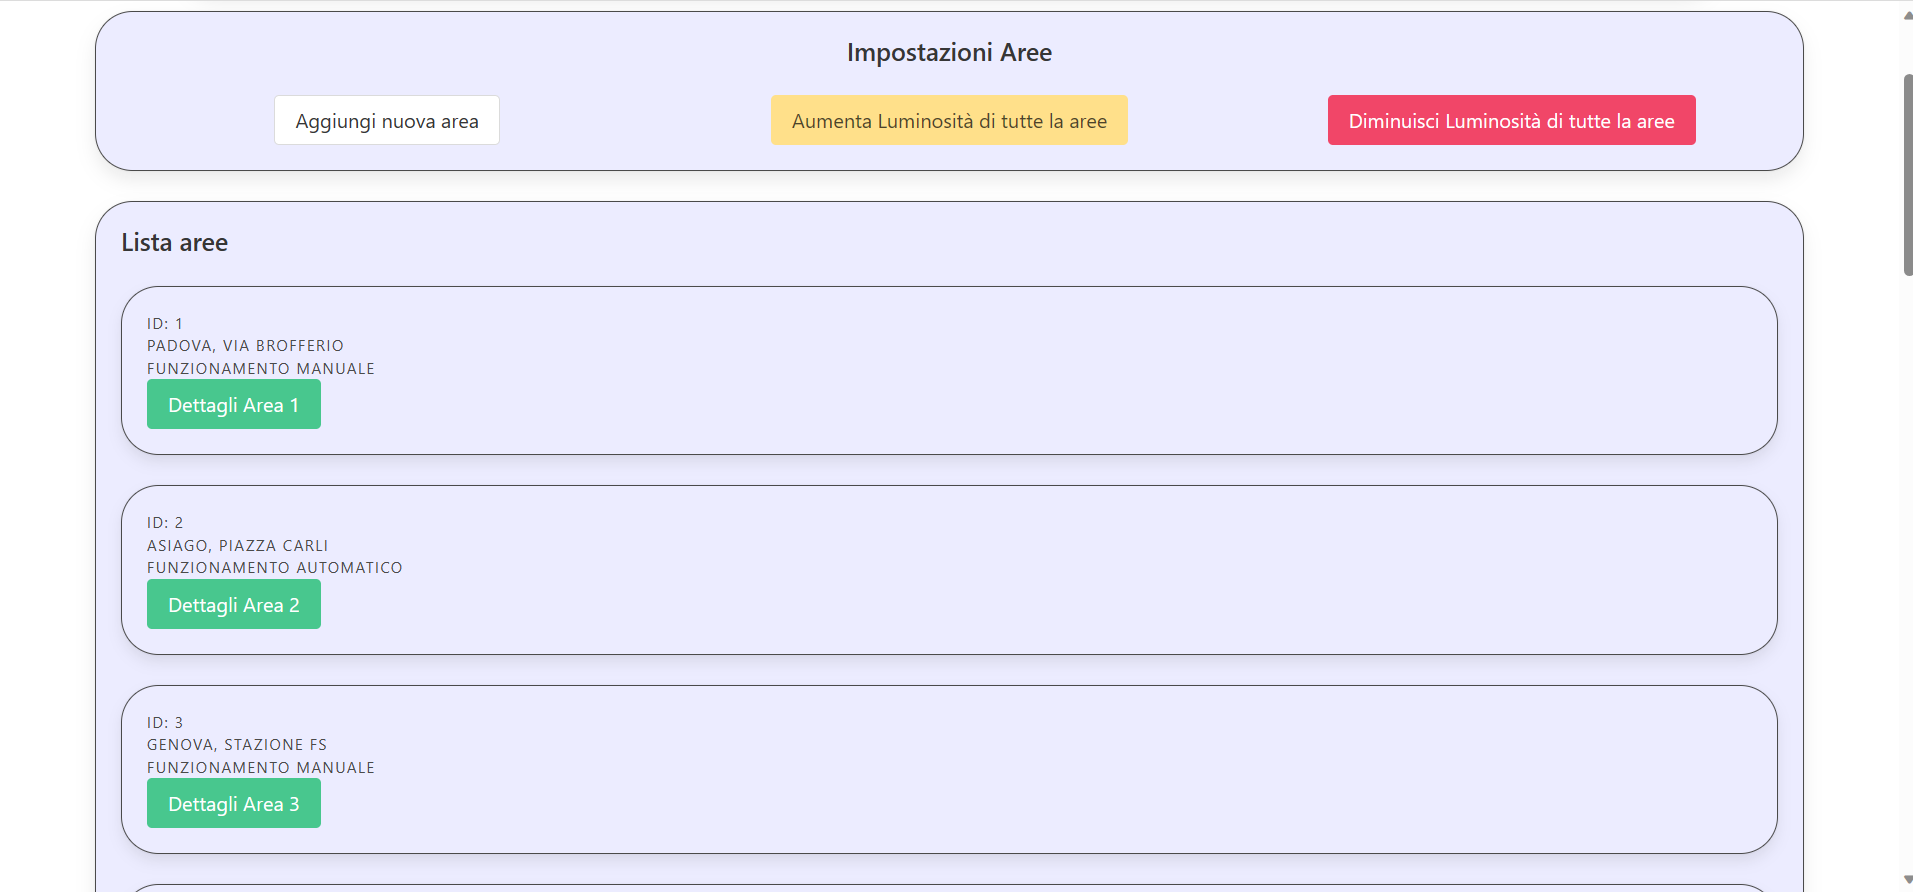
\includegraphics[scale=0.3]{Gestione_aree.png}
\end{center}

Nella sezione "Impostazioni Aree" è presente il tasto per aggiungere una nuova area di illuminazione, che porterà alla pagina "Aggiugni area", insieme ai due tasti per aumentare e diminuire la luminosità di tutte le aree gestite in modo automatico.

\subsection{Aggiungi area}

In questa pagina è possibile immettere tutte le informazioni riguardanti l'area illuminata che si vuole inserire.
Le informazioni inseribili sono le seguenti:
\begin{itemize}
	\item nome città: stringa di testo che identifica una città per nome
	\item zona geografica città: stringa di testo che identifica in che area specifica della città si sta inserendo il sistema di gestione di illuminazione. Può essere una via, un insieme di strade o un luogo ben definito, come ad esempio "Prato della Valle".
	\item modalità di funzionamento: si selezioni automatico se non si vuole gestire personalmente il sistema, manuale altrimenti
	\item stato: indica lo stato del sistema
	\item luminosità default: indica la luminosità che il sistema manterrà finchè non si verificheranno rilevamenti dai sensori
	\item luminosità rilevamento: indica la luminosità che il sistema emetterà quando un sensore rileverà la presenza di un veicolo o di un pedone.
\end{itemize}


\begin{center}
	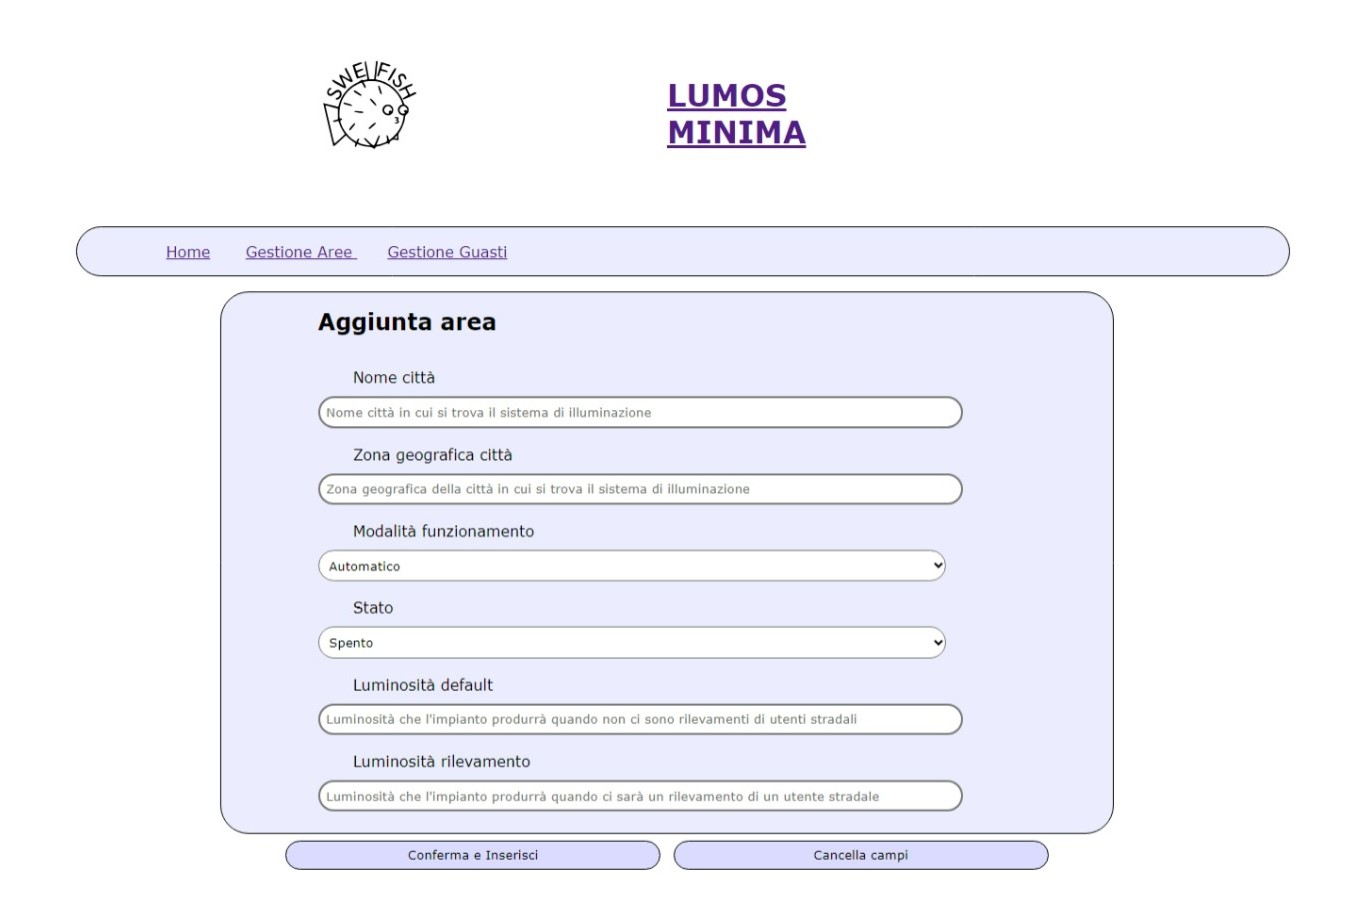
\includegraphics[scale=0.3]{Aggiungi_area.png}
\end{center}

Una volta terminato l'inserimento dei dati, cliccando sul pulsante "Conferma e Inserisci"
l'area verrà inserita nel sistema e si verrà reindirizzati nella pagina "Area" con il dettaglio dell'area appena inserita.\\
Premendo il pulsante cancella campi, le informazioni inserite nel form verranno cancellate e sarà possibile inserirne di nuove.
\subsection{Area}

In questa sezione è possibile gestire tutti gli aspetti legati all'area di illuminazione selezionata

\begin{center}
	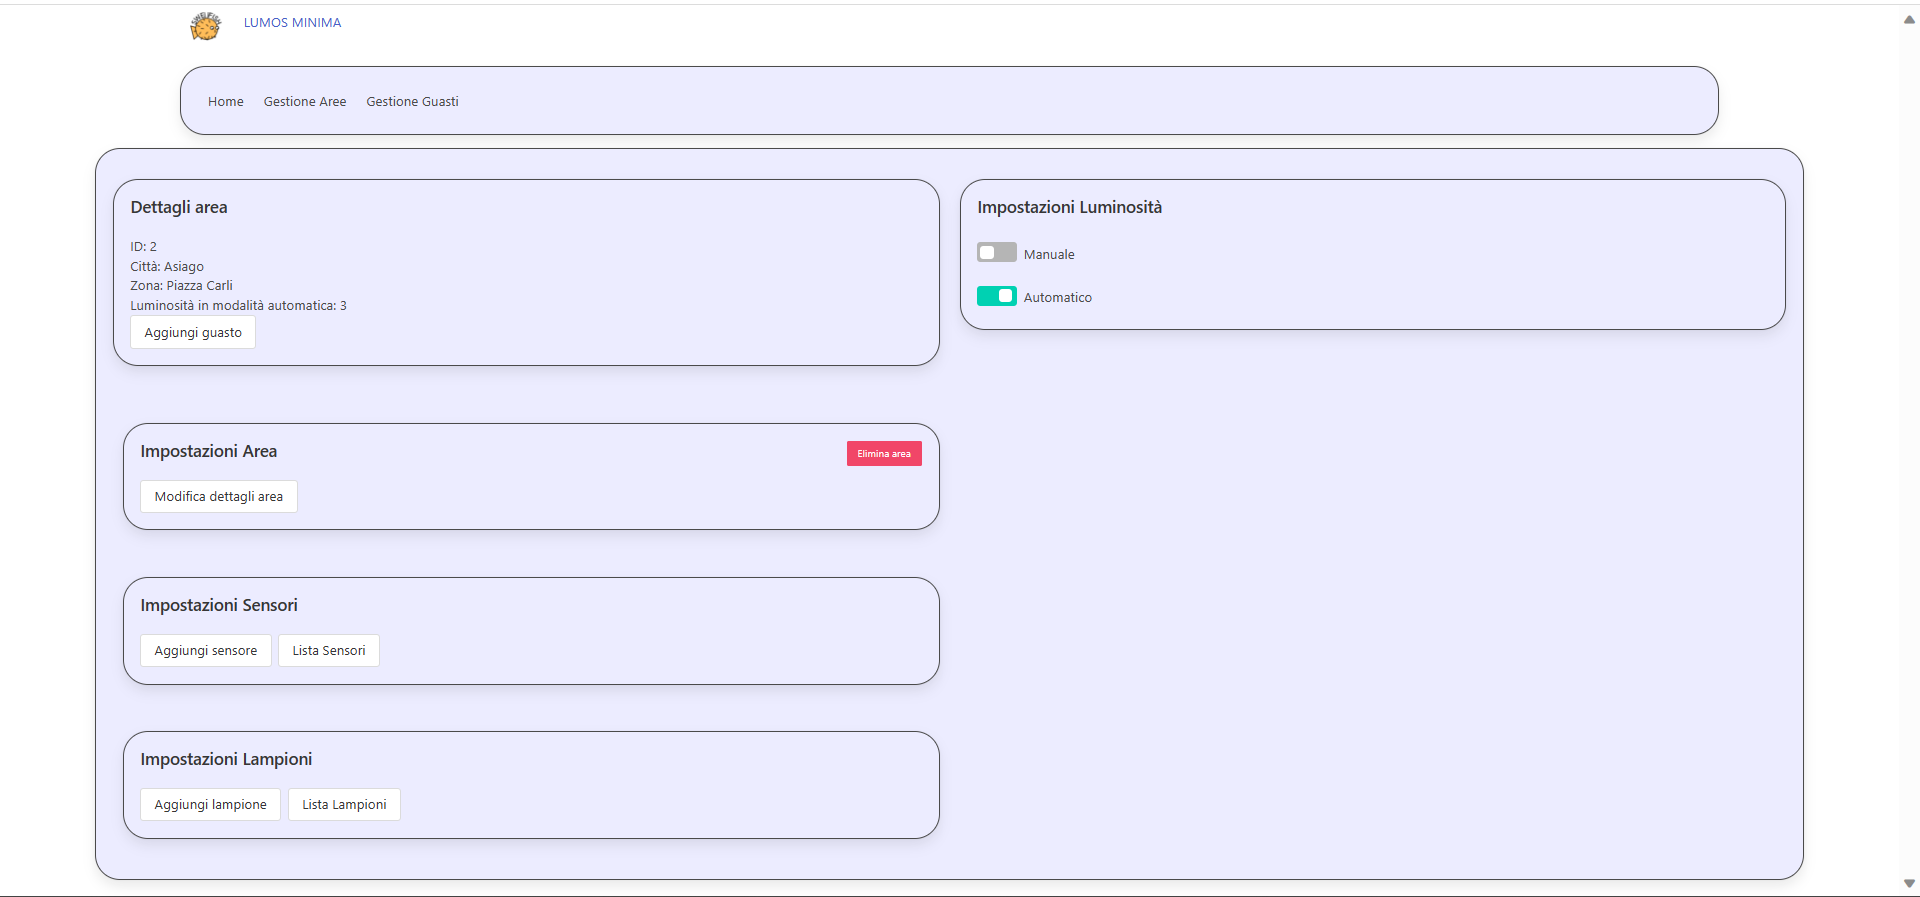
\includegraphics[scale=0.3]{Area.png}
\end{center}

La pagina è suddivisa nei seguenti riquadri:
\begin{itemize}
	\item \textbf{Primo riquadro in alto a sinistra}: Contiene i dettagli dell'area e un pulsante con cui è possibile aggiungere direttamente un guasto associato all'area.
	\item \textbf{Primo riquadro in alto a destra}: Contiene i pulsanti che permettono di gestire l'illuminazione dell'area in maniera manuale oppure automatica.
	\item \textbf{Secondo riquadro a sinistra}: Contiene i pulsanti per l'eliminazione dell'area o per la modifica delle sue informazioni.
	\item \textbf{Terzo riquadro a sinistra}: Contiene i pulsanti per aggiungere un sensore all'area, che porta alla pagina "Aggiungi sensore" e per visualizzare la lista dei sensori dell'area, che porta alla pagina "Lista sensori".
	\item \textbf{Quarto riquadro a sinistra}: Contiene i pulsanti per aggiungere un lampione all'area, che porta alla pagina "Aggiungi lampione" e per visualizzare la lista dei lampioni dell'area, che porta alla pagina "Lista lampioni".
\end{itemize}

\subsection{Aggiungi guasto}
In questa pagina è possibile immettere tutte le informazioni riguardanti il guasto che si vuole inserire.
Le informazioni inseribili sono le seguenti:
\begin{itemize}
	\item Data rilevamento: data in cui il guasto è stato rilevato
	\item Stato: di default un guasto viene segnalato come "Non risolto". 
	\item Note aggiuntive: textbox che permette di inserire dettagli aggiuntivi di interesse per il manutentore.
	\item ID area illuminata afferenza: mostra l'id dell'area a cui viene associato il guasto. Questa informazione non è modificabile.

\begin{center}
	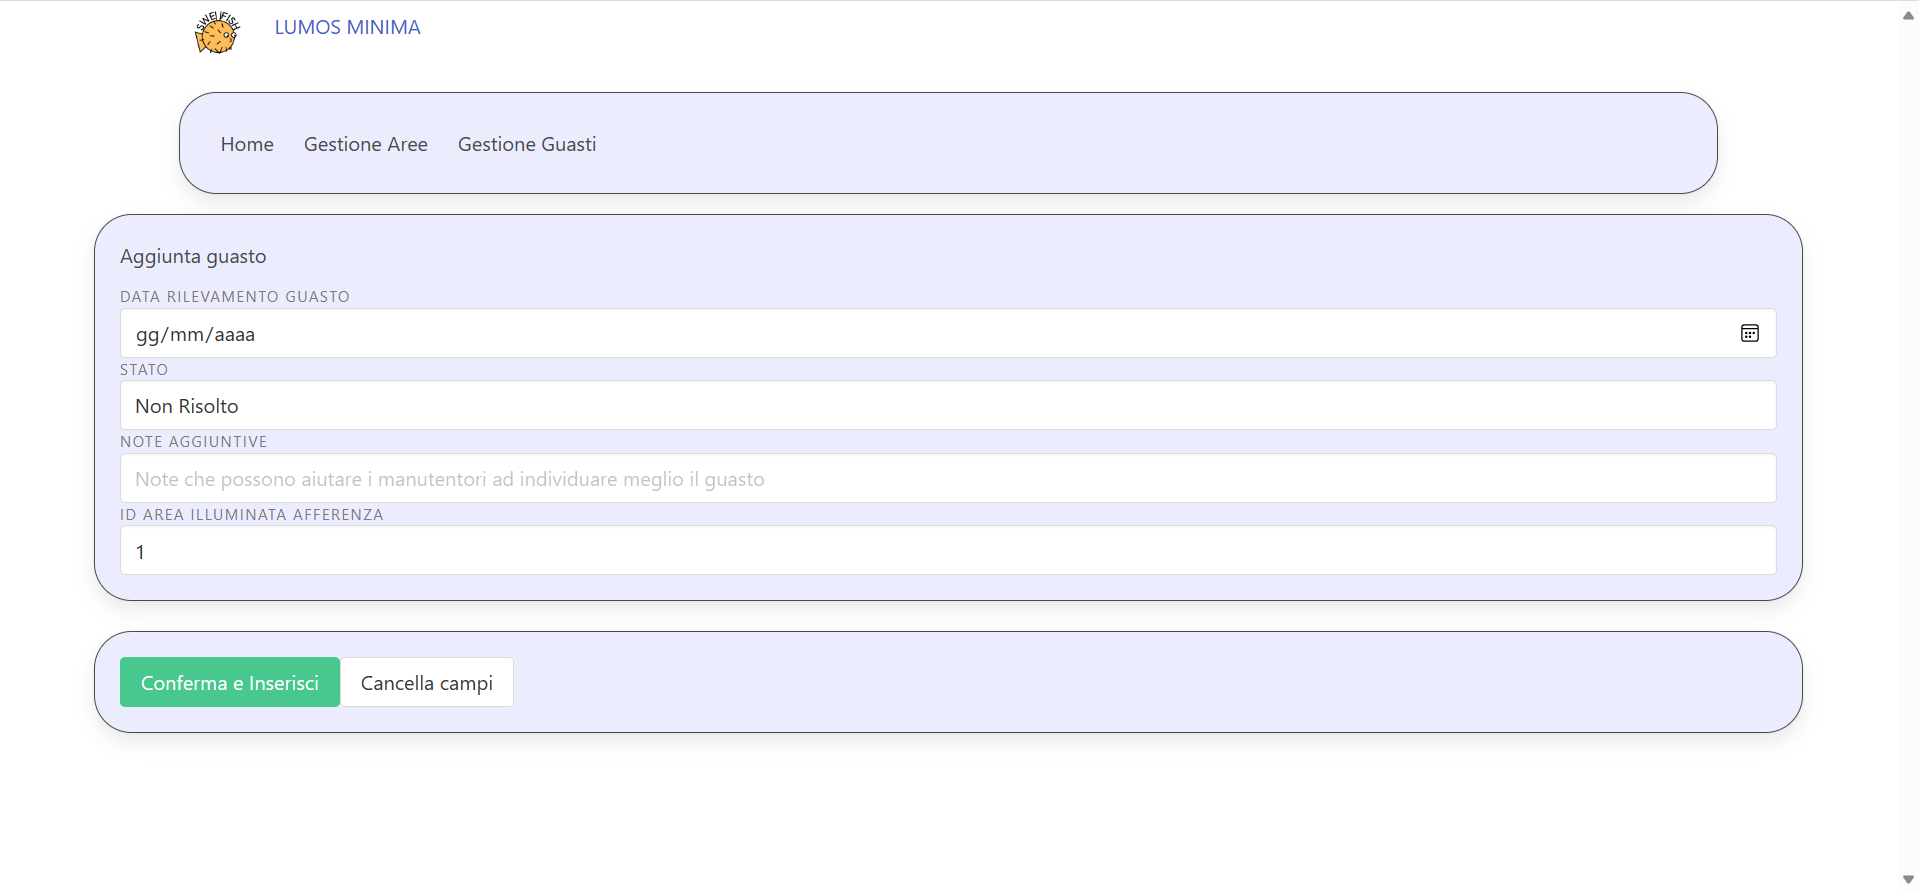
\includegraphics[scale=0.3]{Aggiungi_guasto.png}
\end{center}

Una volta terminato l'inserimento dei dati, cliccando sul pulsante "Conferma e Inserisci"
il guasto verrà inserito nel sistema.


\subsection{Aggiungi sensore}
In questa pagina è possibile immettere tutte le informazioni riguardanti il sensore che si vuole inserire.
I campi dati inseribili sono i seguenti:
\begin{itemize}
	\item indirizzo ip del sensore: stringa di testo che rappresenta l'IP con cui è possibile comunicare con il sensore.
	\item Polling time: tempo in secondi che intercorre tra i vari refresh dello stato del sensore.
	\item zona geografica: luogo esatto in cui è posizionato il sensore
	\item tipo interazione: modalità di interazione del senore, push o pull.
	\item raggio azione: numero di metri entro il quale il sensore è in grado di rilevare la presenza
	\item ID area illuminata afferenza: mostra l'id dell'area a cui viene associato il sensore. Questa informazione non è modificabile
\end{itemize}

\begin{center}
	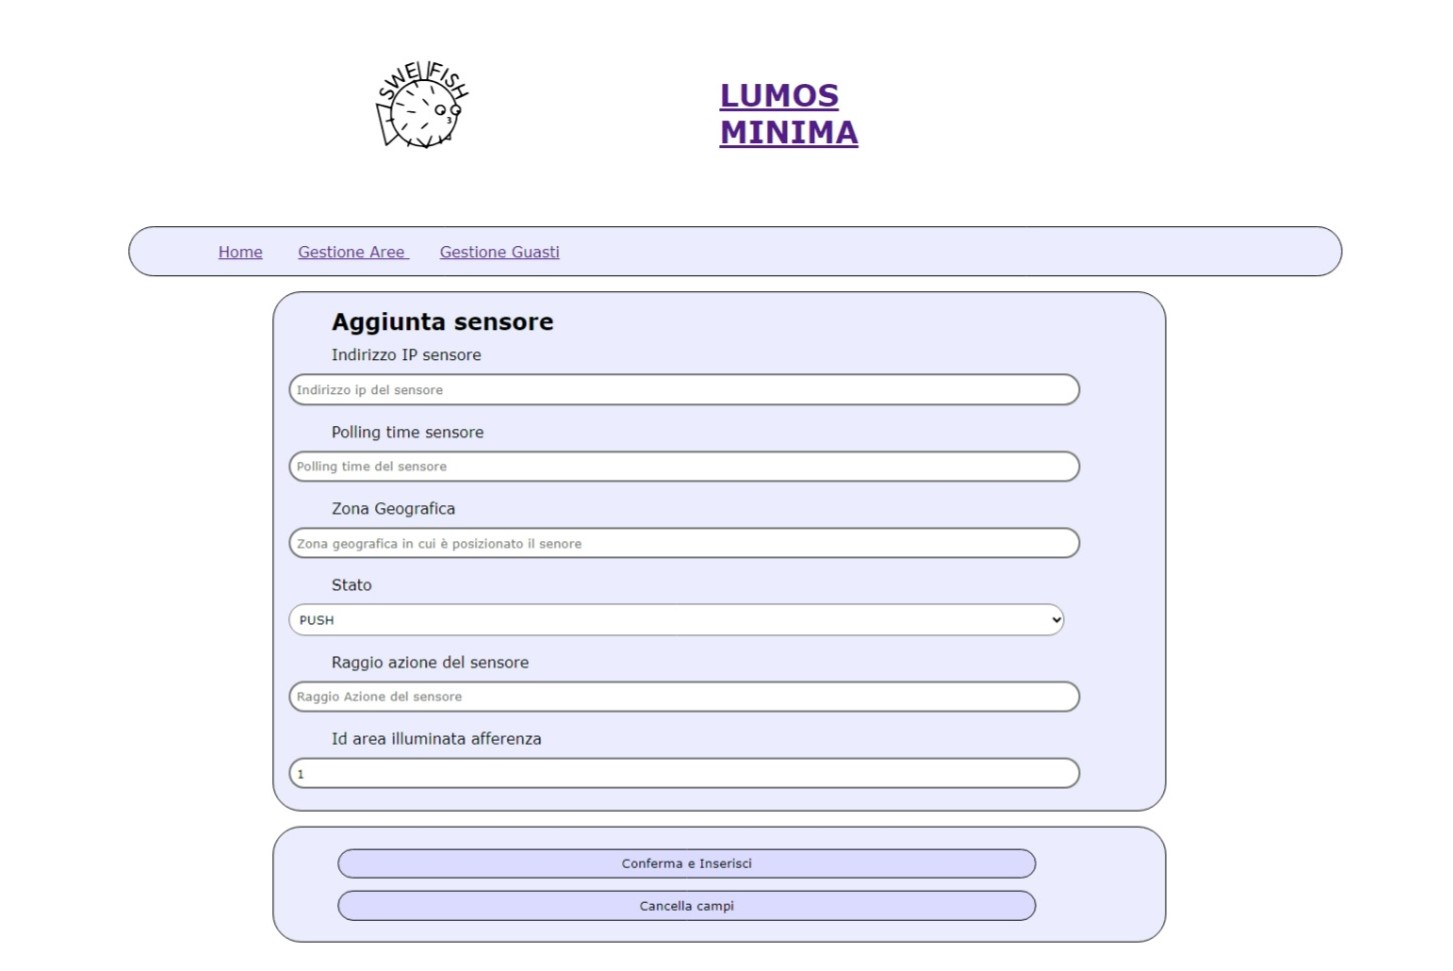
\includegraphics[scale=0.3]{Aggiungi_sensore.png}
\end{center}

Una volta terminato l'inserimento dei dati, cliccando sul pulsante "Conferma e Inserisci"
il sensore verrà inserito nel sistema.

\subsection{Lista sensori}
In questa pagina è presente la lista di tutti i sensori dell'area indicata.
Ogni sensore ha un tasto associato che porta alla pagina di modifica del sensore. 

\begin{center}
	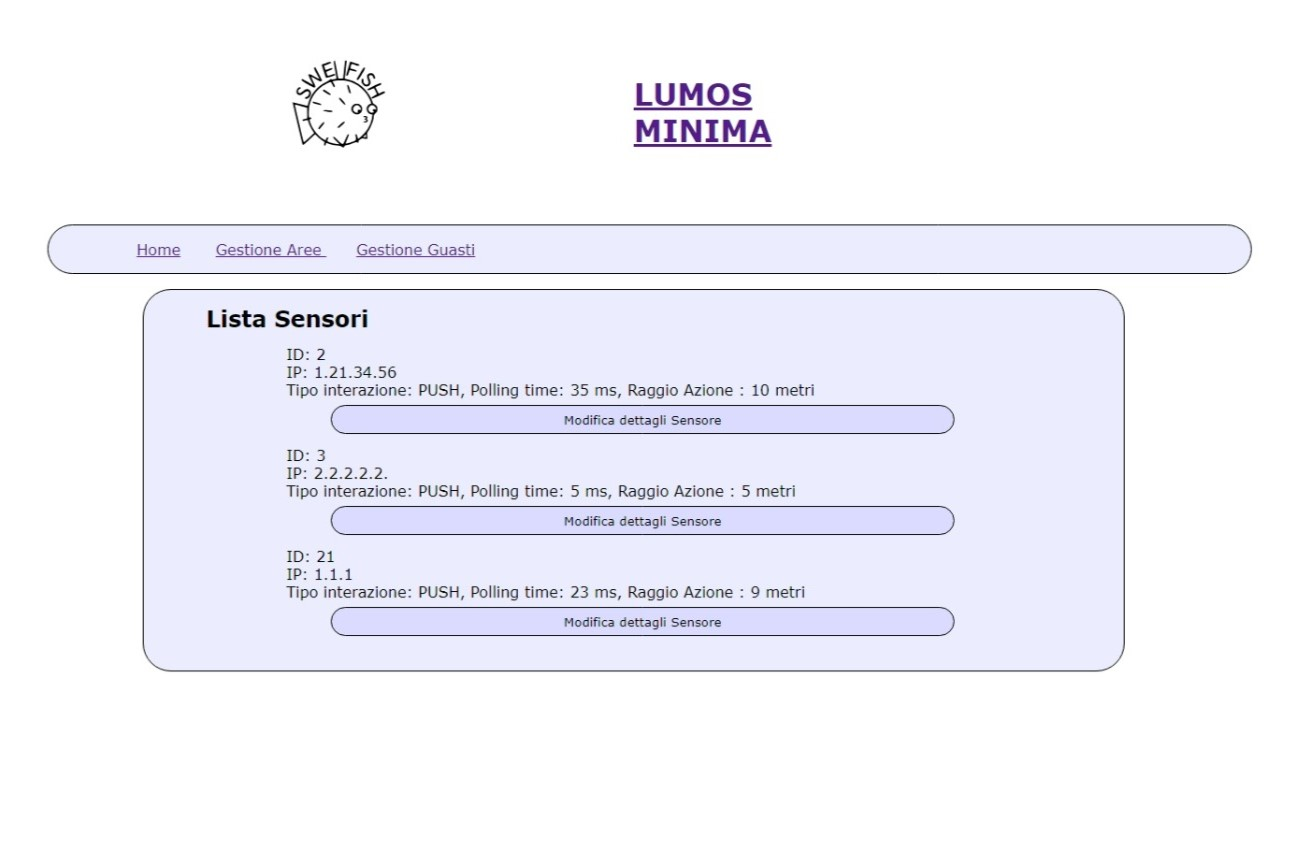
\includegraphics[scale=0.3]{Lista_sensori.png}
\end{center}

\subsection{Modifica sensore}
In questa pagina è possibile immettere tutte le informazioni riguardanti il sensore che si vuole modificare.
I campi dati modificabili sono i seguenti:
\begin{itemize}
	\item indirizzo ip del sensore: stringa di testo che rappresenta l'IP con cui è possibile comunicare con il sensore.
	\item Polling time: tempo in secondi che intercorre tra i vari refresh dello stato del sensore.
	\item zona geografica: luogo esatto in cui è posizionato il sensore
	\item tipo interazione: modalità di interazione del senore, push o pull.
	\item raggio azione: numero di metri entro il quale il sensore è in grado di rilevare la presenza
\end{itemize}

\begin{center}
	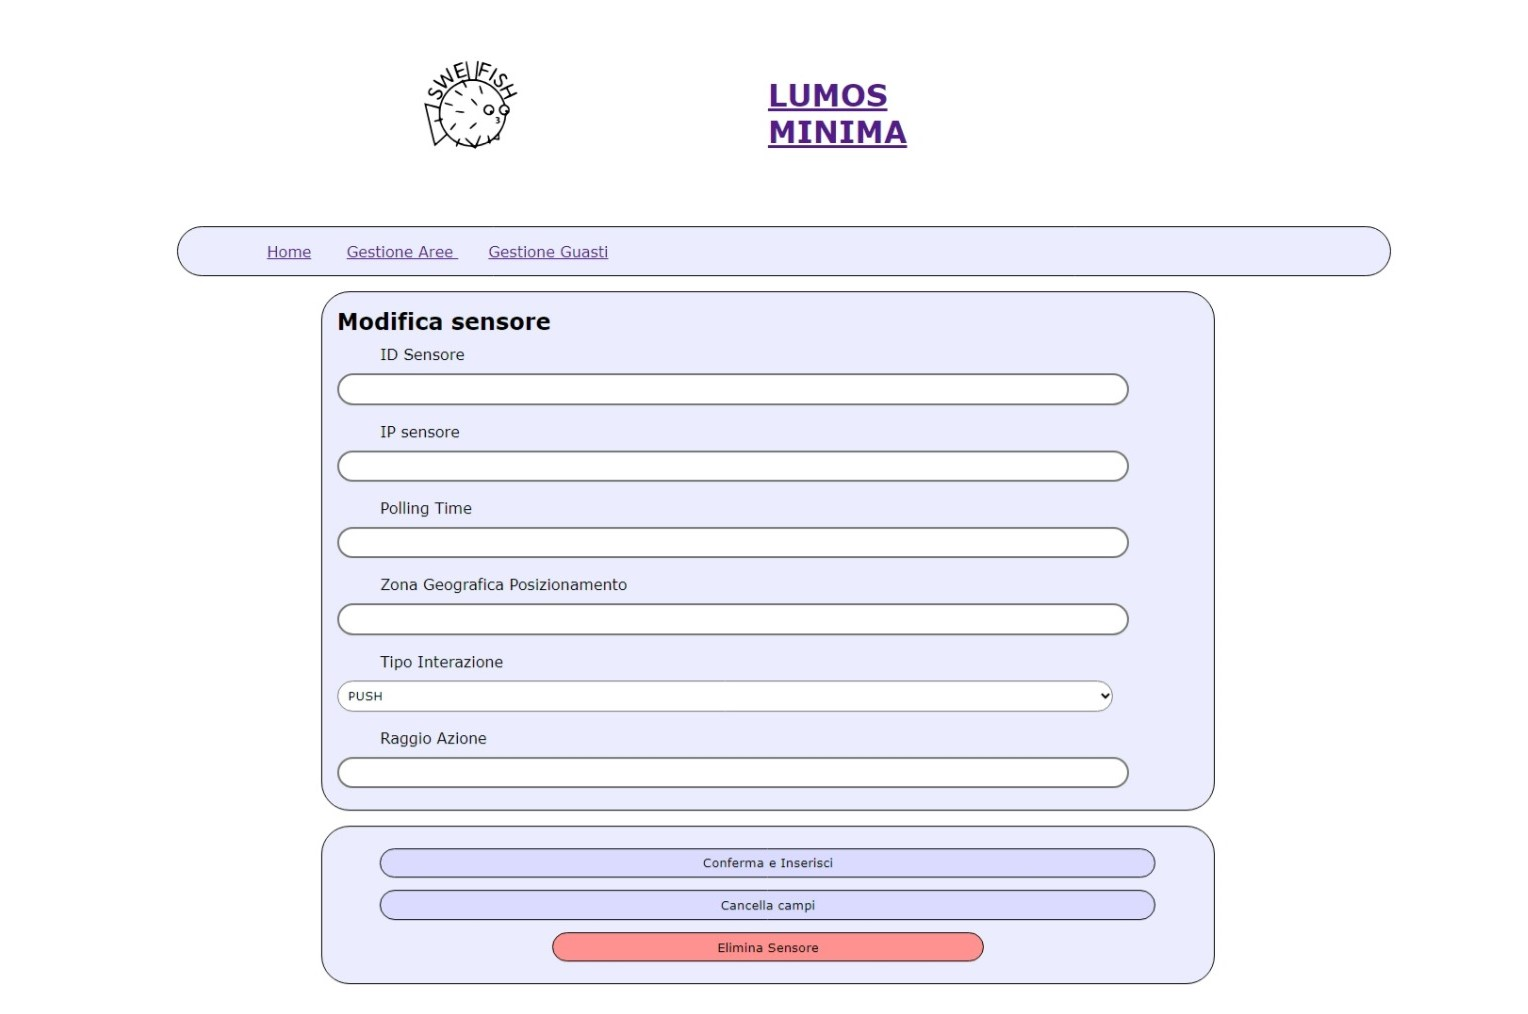
\includegraphics[scale=0.3]{Modifica_sensore.png}
\end{center}

Una volta terminato l'inserimento dei dati, cliccando sul pulsante "Conferma e Inserisci"
la modifica verrà inserita nel sistema.
E' anche presente il tasto per eliminare il sensore dal sistema.


\subsection{Aggiungi lampione}
In questa pagina è possibile immettere tutte le informazioni riguardanti il lampione che si vuole inserire.
I campi dati inseribili sono i seguenti:
\begin{itemize}
	\item indirizzo ip del lampione: stringa di testo che rappresenta l'IP con cui è possibile comunicare con il lampione.
	\item tipo interazione: modalità di interazione del lampione, push o pull.
	\item luminosità manuale: luminosità che il lampione produrrà quando comandato singolarmente
	\item stato: acceso o spento. Questa impostazione si riferisce al funzionamento manuale per singolo lampione.
	\item ID area illuminata afferenza: mostra l'id dell'area a cui viene associato il lampione. Questa informazione non è modificabile
\end{itemize}


\begin{center}
	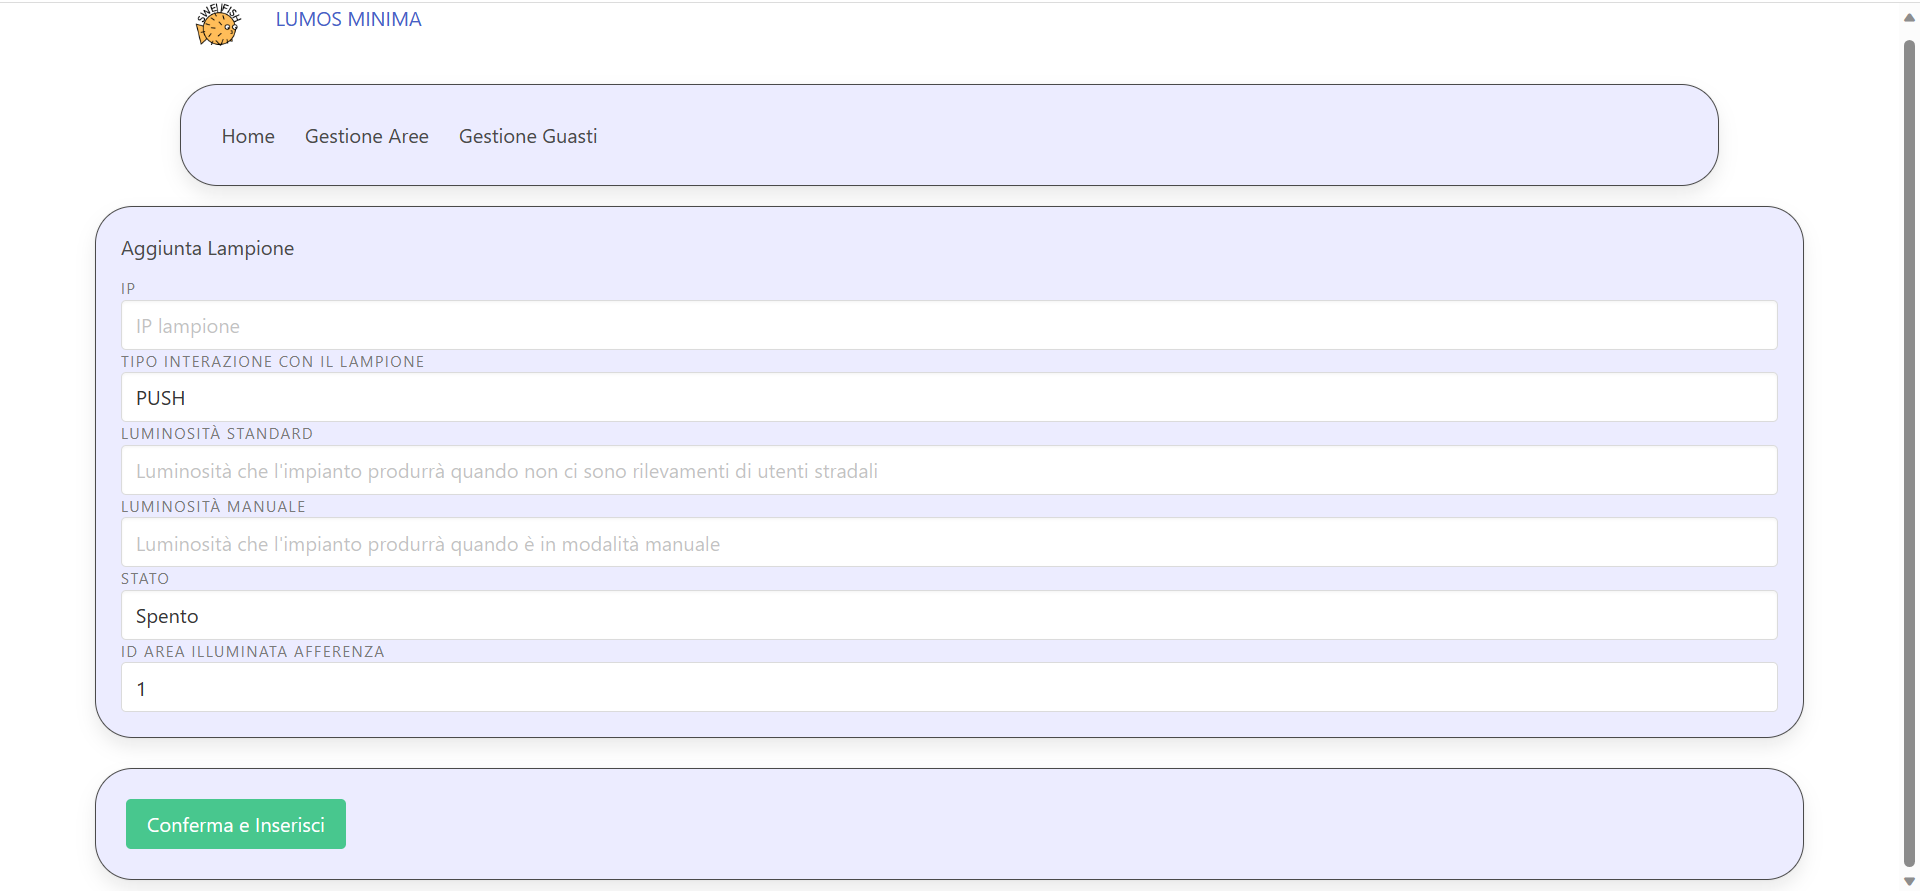
\includegraphics[scale=0.3]{Aggiungi_lampione.png}
\end{center}

Una volta terminato l'inserimento dei dati, cliccando sul pulsante "Conferma e Inserisci"
il lampione verrà inserito nel sistema.

\subsection{Lista lampioni}
In questa pagina è presente la lista di tutti i lampioni dell'area indicata.
Ogni lampione ha un tasto associato per spegnerlo e uno che porta alla pagina di modifica del lampione.

\begin{center}
	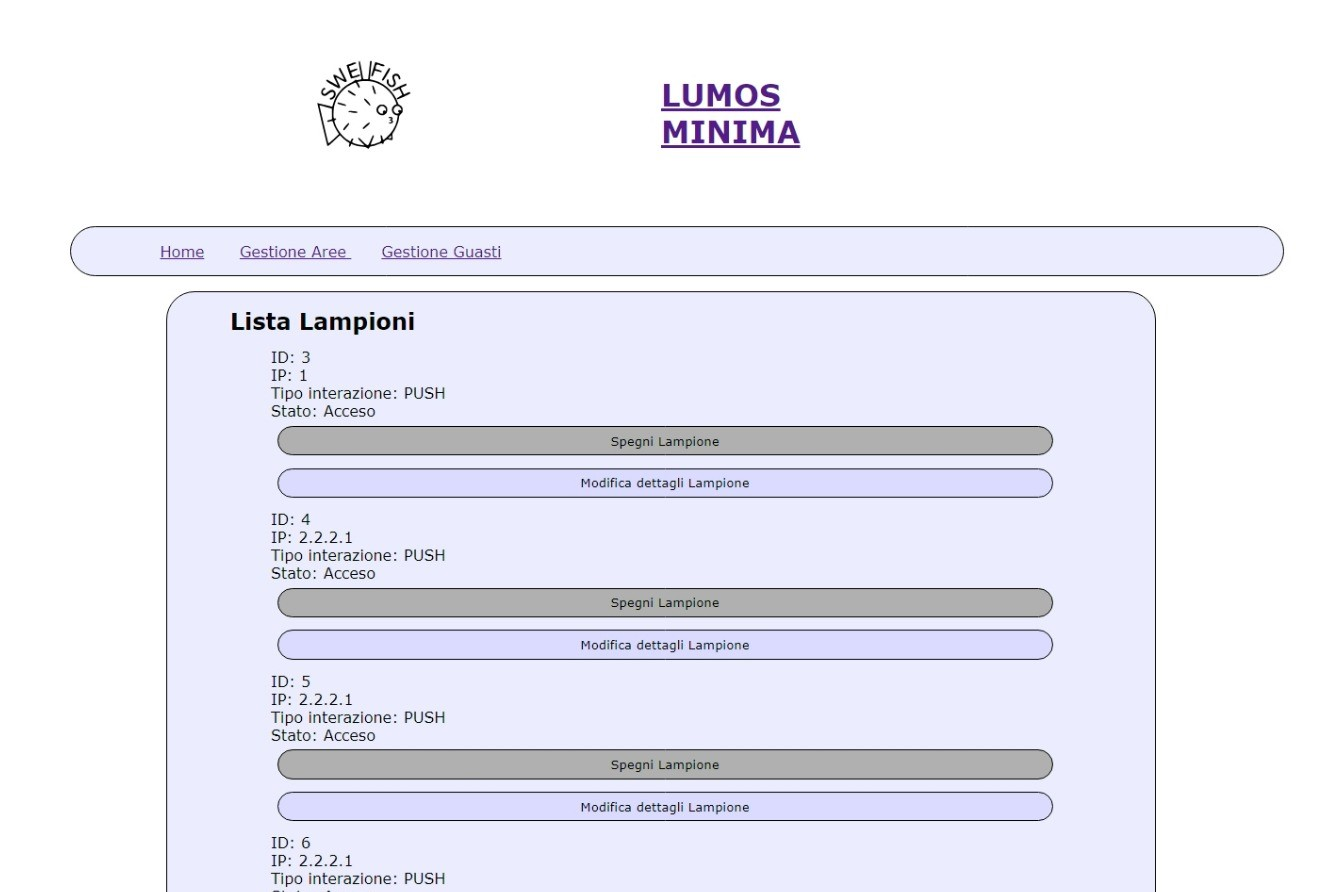
\includegraphics[scale=0.3]{Lista_lampioni.png}
\end{center}


\subsection{Modifica lampione}
In questa pagina è possibile immettere tutte le informazioni riguardanti il lampione che si vuole modificare.
I campi dati modificabili sono i seguenti:
\begin{itemize}
	\item indirizzo ip del lampione: stringa di testo che rappresenta l'IP con cui è possibile comunicare con il lampione.
	\item tipo interazione: modalità di interazione del lampione, push o pull.
	\item luminosità manuale: luminosità che il lampione produrrà quando comandato singolarmente
	\item stato: acceso o spento. Questa impostazione si riferisce al funzionamento manuale per singolo lampione.
\end{itemize}


\begin{center}
	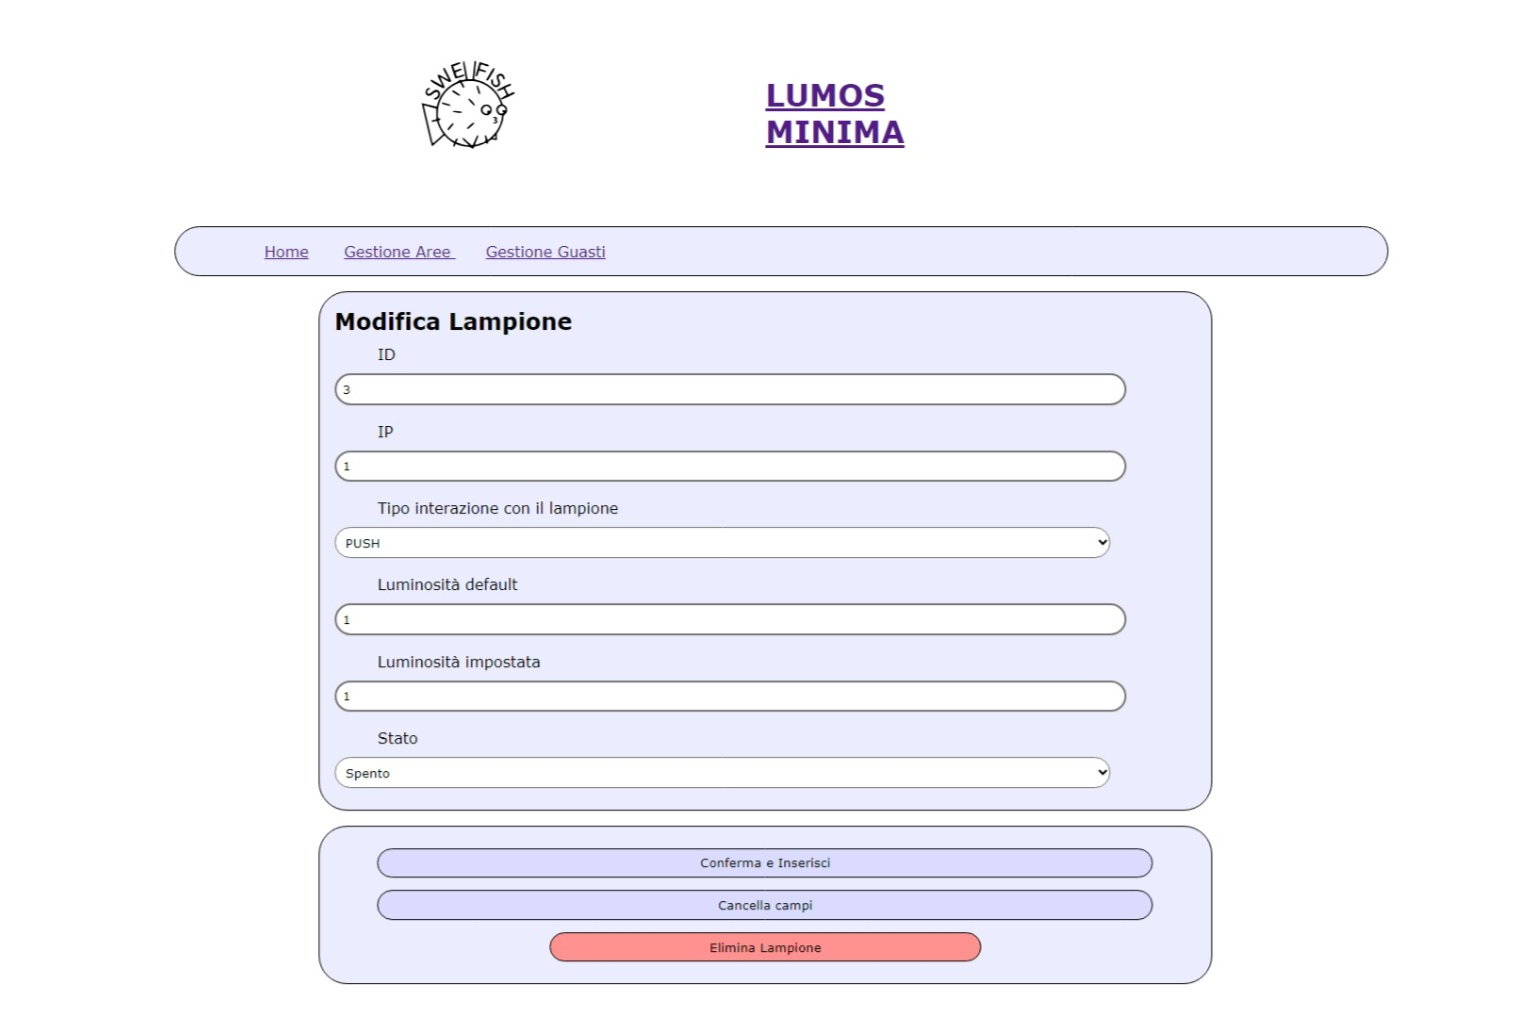
\includegraphics[scale=0.3]{Modifica_lampione.png}
\end{center}

Una volta terminato l'inserimento dei dati, cliccando sul pulsante "Conferma e Inserisci"
la modifica verrà inserita nel sistema.
E' anche presente il tasto per eliminare il lampione dal sistema.


\subsection{Gestione guasti}
In questa pagina è presente la lista di tutti i guasti inseriti a sistema.
I guasti vengono suddivisi automaticamente in guasti aperti, ovvero non ancora risolti e guasti chiusi, ovvero guasti risolti.
Ogni guasto ha un tasto associato che porta alla pagina di dettaglio corrispondente al guasto cliccato.

\begin{center}
	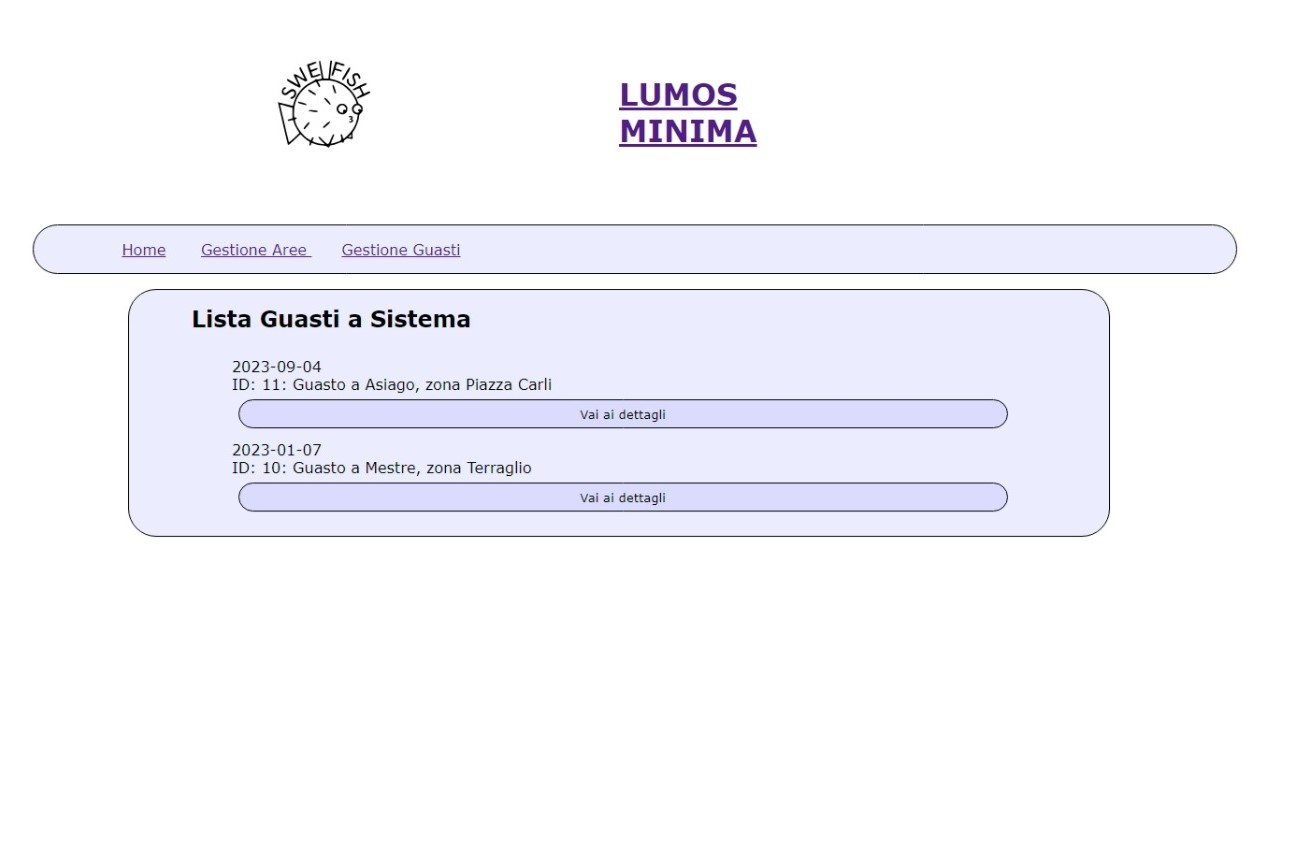
\includegraphics[scale=0.3]{Gestione_guasti.png}
\end{center}

\subsection{Guasto}

In questa pagina è possibile gestire tutti gli aspetti legati al guasto selezionato.

\begin{center}
	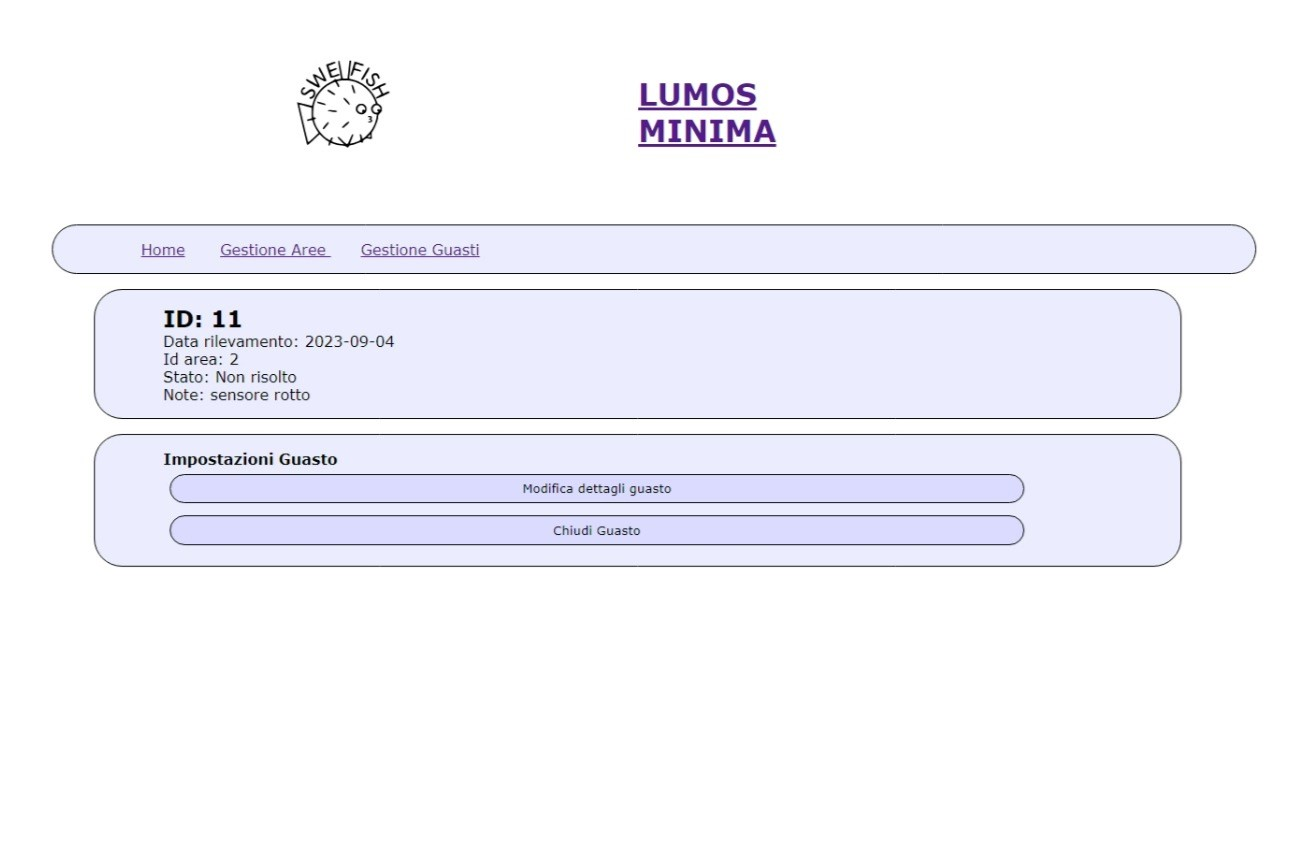
\includegraphics[scale=0.3]{Guasto.png}
\end{center}

La pagina è suddivisa nei seguenti riquadri:
\begin{itemize}
	\item \textbf{la sezione 1}: Informazioni contententi i dettagli del guasto.
	\item \textbf{la sezione 2}: Pulsanti per la chiusura del guasto o per la modifica delle sue informazioni.
\end{itemize}

\subsection{Modifica guasto}
In questa pagina è possibile immettere tutte le informazioni riguardanti il guasto non risolto che si vuole modificare.
I dati modificabili sono i seguenti:
\begin{itemize}
	\item stato: è possibile segnalare la chiusura del guasto direttamente da questa sezione.
	\item Note aggiuntive: le note a supporto del manutentore sono modificabili direttamente da questa sezione.
\end{itemize}

\begin{center}
	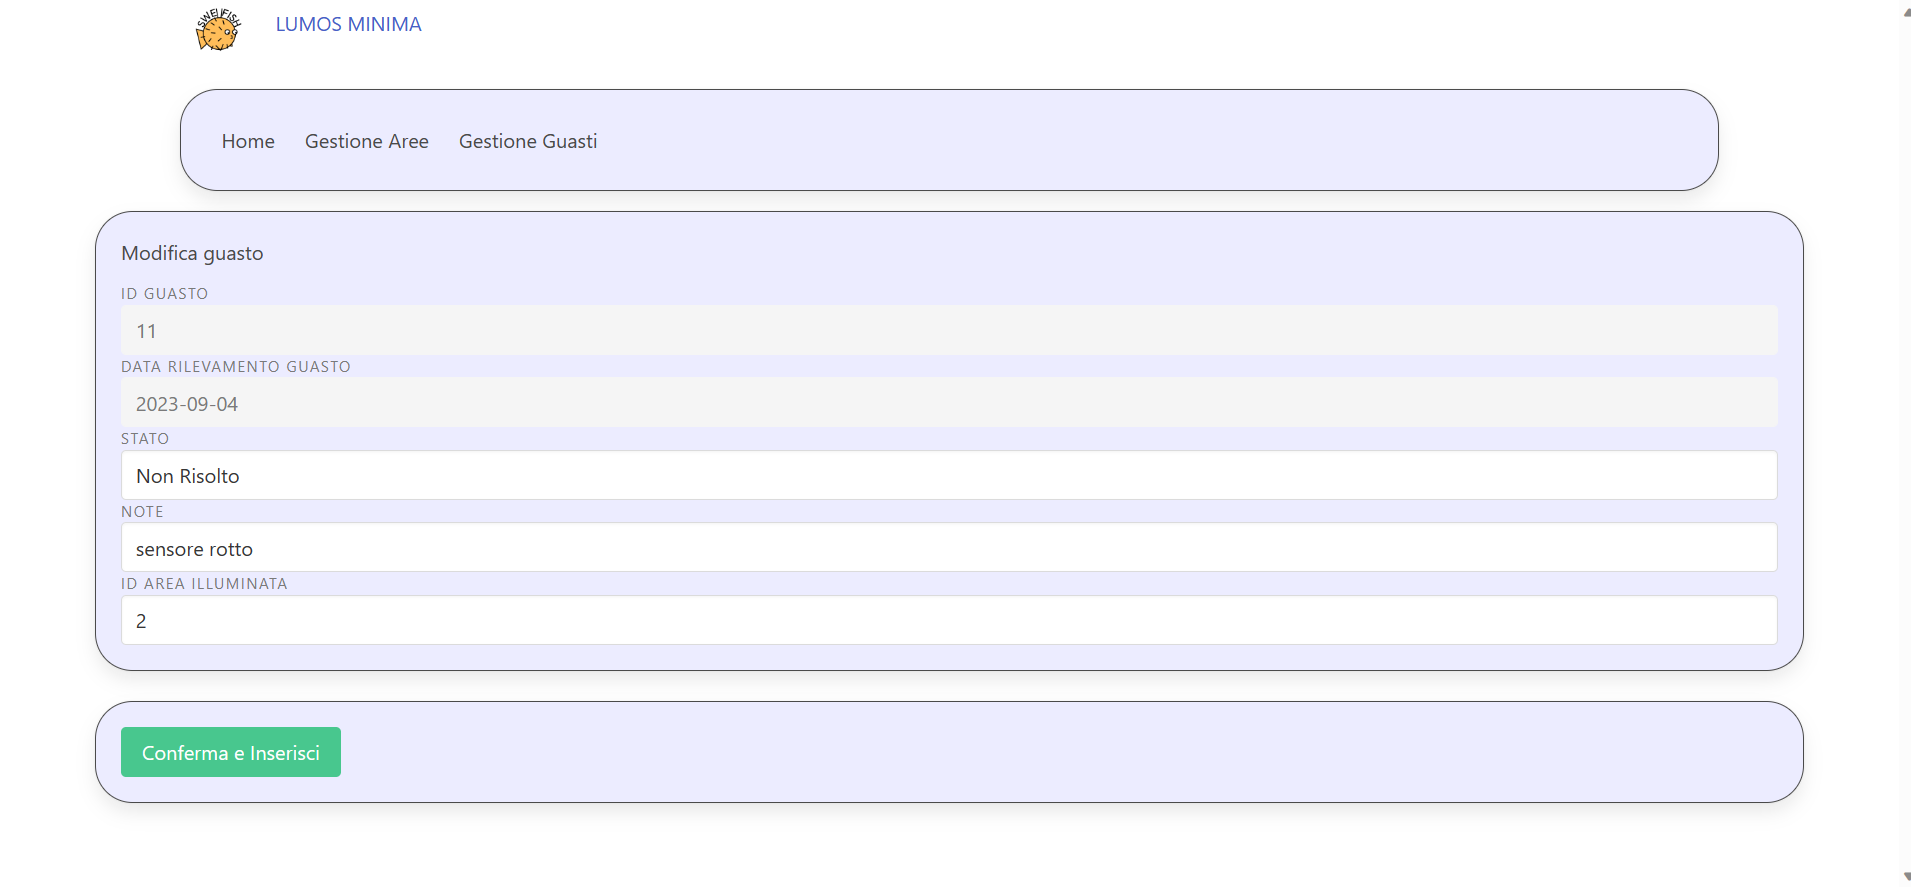
\includegraphics[scale=0.3]{Modifica_guasto.png}
\end{center}

Una volta terminato l'inserimento dei dati, cliccando sul pulsante "Conferma e Inserisci"
la modifica verrà inserita nel sistema.



\end{document}
